\documentclass{article}
\usepackage{graphicx}
\begin{document}
\title{Como usuario, me gustaría jugar a Rolit pensando en las posibilidades que brinda el multijugador (Red)}
\maketitle
\section*{Sprint 5}
En cuanto a la tarea de añadir un modo de juego en red, se concibe, planea e implementa la funcionalidad de red casi por completo, consigue llegar a una versión funcional de juego en red en GameClassic. Al final del Sprint, los objetivos alcanzados son los siguientes:

\begin{itemize}
\item Determinar si el servidor, o por el contrario el cliente, debería poseer el modelo. Optamos por la segunda opción.

\item Definir toda la estructura en cuanto a relaciones jerárquicas de clases y dependencias entre las mismas. Al diagrama UML de clases llegado fue el siguiente:

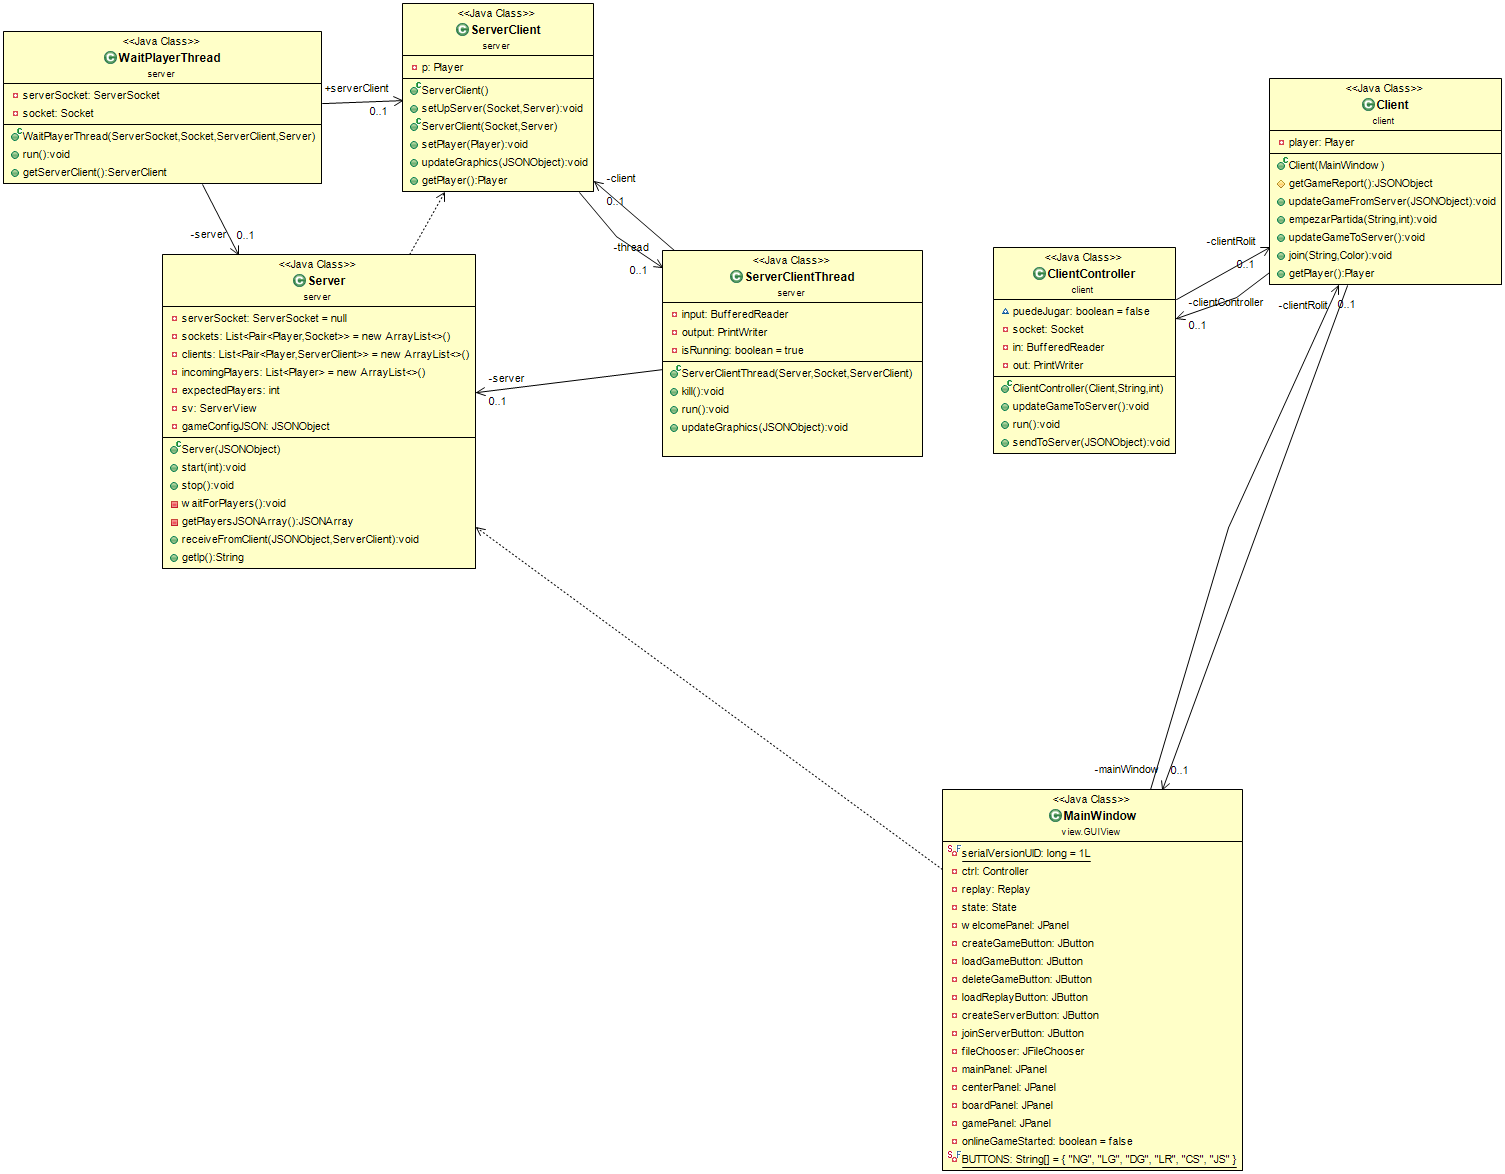
\includegraphics[scale=0.25]{UMLClasesRedSprint5.png} 

\item Crear un número suficiente de diálogos en GUI que permitan la conexión en red. Entre ellos, se encuentran:
\begin{itemize}
\item ServerView
\item JoinServerDialog
\end{itemize}

\item Reutilizamiento del código del diálogo de crear partida, adaptado a las circunstancias de red.

\item Poder jugar a una partida GameClassic en red de forma satisfactoria.

\end{itemize}

Aun así, otros de los objetivos propuestos no son implementados por falta de tiempo y de dependencia con otras de las partes del desarrollo no concluidos. Estos objetivos son:

\begin{itemize}
\item Crear más diálogos que aporten feedback para la conexión, tanto de la perspectiva del cliente como del servidor.

\item Llegar a una versión completamente refactorizada y con métodos simplificados.

\item Implementar el juego en red en GameTeams.
\end{itemize}

El hilo de ejecución típico de una partida es el siguiente:

(INSERTAR DIAGRAMAS DE SECUENCIA UML)

\section*{Sprint 6}
En cuanto a la red, se alcanzan los objetivos propuestos que quedaron pendientes en el Sprint 5. Las características implementadas son:

\begin{itemize}
\item Implementación del modo red para GameTeams.

\item Creación de diálogos y de código auxiliar para soportar GameTeams.

\begin{itemize}
\item Una clase creada para tal efecto es ChooseTeamFromServerDialog.
\end{itemize}


\item Perfeccionamiento de la estructura y relaciones de las comunicaciones cliente-servidor y viceversa, incluyendo mecanismos como un campo en el JSON mensaje que especifica qué tipo de notificación constituye el mensaje enviado.

\item Adaptación de los diálogos GUI de red al nuevo diseño de la interfaz gráfica introducido en este Sprint.

\item Se introduce un ServerWorker que soluciona un bug complejo que afectaba a los threads de Red y Swing.

\item Simplificación y refactorización del código de Red.

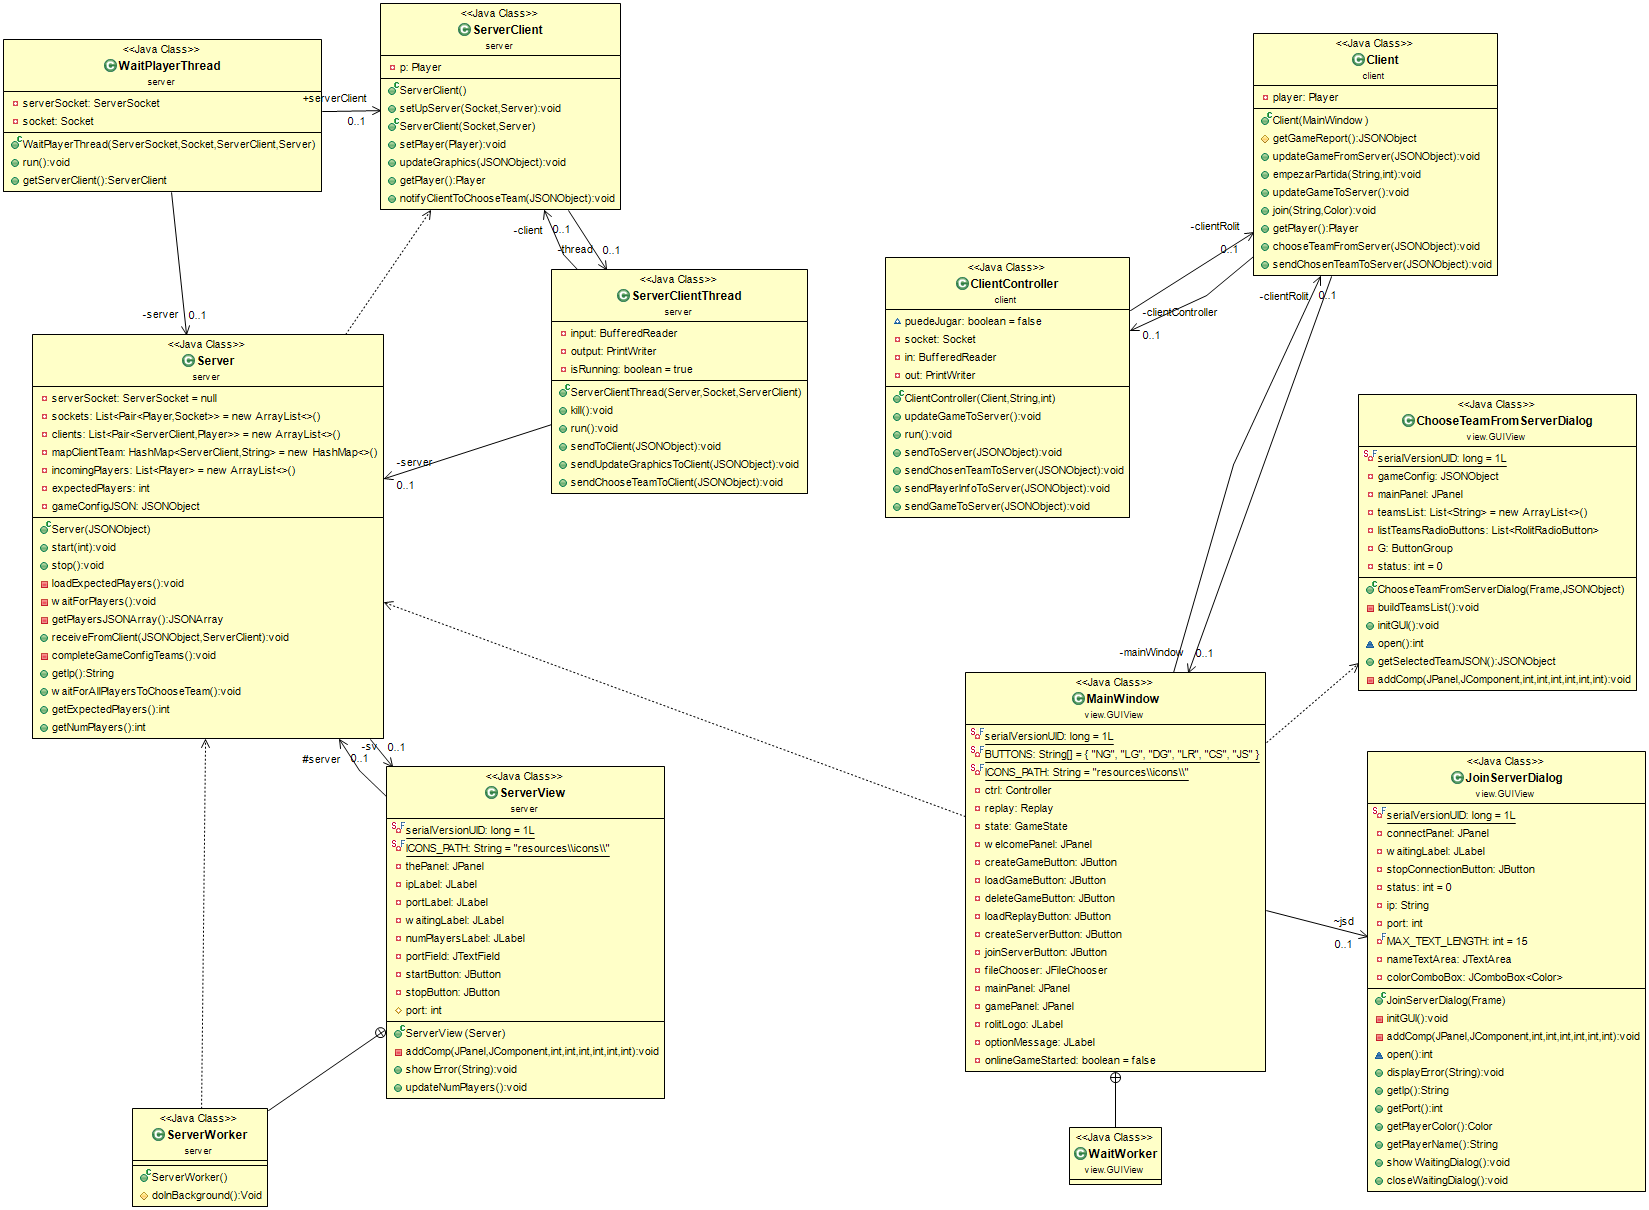
\includegraphics[scale=0.25]{UMLClasesRedSprint6.png} 

\end{itemize}

Por último las sucesivas refactorizaciones pugnadas desde otras partes del código (para, por ejemplo soportar la IA) precisan de un debug extensivo en el modo Red. Este debug es satisfactorio.

(INSERTAR DIAGRAMAS DE SECUENCIA UML)

\section*{Sprint 7}

En cuanto a la red, si bien está conclusa llegados a este Sprint, el debug realizado en otras zonas del código influyen directamente en la funcionalidad de Red. Se lleva a cabo un debug rápido pero extensivo para verificar que el modo de juego en red no ha sido afectado, llevándose a cabo con éxito.

Por último, se procede a crear y solventar algunas issues relativas a la experiencia de usuario jugando en red, conllevando una serie de modificaciones que hacen más intuitiva las instrucciones para realizar la conexión.
\end{document}